\documentclass[conference]{IEEEtran}
\IEEEoverridecommandlockouts
% The preceding line is only needed to identify funding in the first footnote. If that is unneeded, please comment it out.
\usepackage{cite}
\usepackage{amsmath,amssymb,amsfonts}
\usepackage{algorithmic}
\usepackage{graphicx}
\usepackage{listings}
\lstset{breaklines=true}
\usepackage{url}
\usepackage{hyperref}
\usepackage{dirtree}
\graphicspath{ {images/} }
\usepackage{textcomp}
\usepackage{xcolor}
\usepackage{todonotes}
\usepackage{subcaption}
\usepackage{placeins}
\usepackage{comment}

\usepackage{tikz}
\usetikzlibrary{calc, patterns, patterns.meta, shapes.geometric, arrows.meta, positioning, fit, decorations.pathreplacing, trees, arrows, shapes.misc, angles, quotes}
%Go-kart command \gokart{"x"}{"y"}{"rot_in_deg"}
\def\gokart#1#2#3{
    \begin{scope}[shift={(#1,#2)}, rotate=#3]
        \begin{scope}[shift={(0,-0.85)}] %Offset so (x,y) is the front bumper
            %Front bumper
            \draw[very thick] (-0.7, 0.75) -- (-0.5, 0.85) -- (0.5, 0.85) -- (0.7, 0.75);
            %Body
            \draw[fill=gray!30] (-0.5,-0.75) rectangle (0.5,0.75);
            %Wheels
            \draw[fill=black, rounded corners=0.75] (-0.6,0.6) rectangle (-0.4, 0.3); % Front left
            \draw[fill=black, rounded corners=0.75] (0.6,0.6) rectangle (0.4, 0.3); % Front right
            \draw[fill=black, rounded corners=0.75] (-0.6,-0.6) rectangle (-0.4, -0.3); % Rear left
            \draw[fill=black, rounded corners=0.75] (0.6,-0.6) rectangle (0.4, -0.3); % Rear right
            %Rear bumper
            \draw[very thick] (-0.6, -0.75) -- (-0.5, -0.8) -- (0.5, -0.8) -- (0.6, -0.75);
        \end{scope}
    \end{scope}
}


\usepackage{siunitx} 
\sisetup{locale = US}
\DeclareSIUnit{\Bit}{Bit}
\DeclareSIUnit{\baud}{Baud}
\DeclareSIUnit{\frame}{f}

\def\BibTeX{{\rm B\kern-.05em{\sc i\kern-.025em b}\kern-.08em
    T\kern-.1667em\lower.7ex\hbox{E}\kern-.125emX}}


\pagestyle{plain}

\begin{document}

\title{Radar odometry using mmWave technology for SLAM applications.\\
{\large Leveraging mmWave Radar Sensor Technology for odometry estimation.}
}

\author{\IEEEauthorblockN{Luis Fernando Rodriguez Gutierrez}
\IEEEauthorblockA{\textit{Fachhochschule Dortmund} \\
\textit{M.Eng. Embedded Systems Engineering}\\
luis.rodriguez001@stud.fh-dortmund.de}

}


\maketitle


\begin{abstract}
Radar technologies have recently emerged as a promising alternative to traditional odometry methods, which often rely on cameras, LiDAR, wheel encoders, inertial sensors, or GPS.  
Unlike these modalities, millimeter-wave (mmWave) radar offers robustness under adverse conditions such as fog, rain, or low light, while directly providing both range and Doppler velocity measurements.  
Previous work has demonstrated that radar can support odometry through global iterative closest point (ICP) alignment of point clouds.  
Building on this foundation, this work focuses on ego-motion estimation using a dual mmWave radar system complemented by an inertial sensor.  
The dual-radar configuration is designed to increase spatial coverage and reduce ambiguity in radar detections, addressing a key limitation of single-radar odometry approaches.  

Experimental evaluations were conducted in both enclosed environments (laboratory) and open environments (university parking lot).  
Results show that the proposed framework provides consistent and reliable ego-motion estimation, highlighting the potential of mmWave radar as a cost-efficient substitute or complement to conventional odometry sources in autonomous navigation.  
\end{abstract}

\begin{IEEEkeywords}
Radar Odometry, mmWave Radar, Dual-Radar Configuration, Clustering, ICP, Doppler Velocity, Submap Aggregation, Ego-Motion Estimation
\end{IEEEkeywords}

\section{Introduction}
\label{sec:intoduction}

Accurate and reliable ego-motion estimation is a fundamental requirement for mobile robotic systems and autonomous vehicles solutions.

Traditionally or in most scenarios, this task has been accomplished using a combination of wheel encoders, inertial measurement units (IMUs), and GPS.
In the most recent years, odometry has been implemented using vision (cameras) or LiDAR-based sensors, which offer dense information about the environment.
However, these modalities often suffer from high cost and performance degradation under adverse conditions such as low illumination, fog, rain, or snow.
As a result of this performance degradation, the accuracy and robustness of odometry are significantly limited and reduced, raising the demand for complementary sensing solutions which may offer a more robust solution in such scenarios.

Odometry provides the basis for localization, mapping, and navigation, serving as a core component in modern perception solutions.  
In most scenarios, odometry has been implemented using vision- or LiDAR-based sensors, which offer dense information about the environment.  
However, these modalities often suffer from performance degradation from high memory consumption and being under adverse conditions such as low illumination, fog, rain, or snow.  
In such scenarios, the accuracy and robustness of odometry are significantly limited and reduced, raising the demand for complementary sensing solutions.  

Millimeter-wave (mmWave) radar has emerged as a promising candidate to address these challenges. Due to its resilience to environmental variability, low cost and native capability to measure both range and veloticy.
Radar sensors are compact, cost-efficient, and resilient to weather and lighting variations, making them attractive for robotic and automotive applications.  
Unlike vision or LiDAR, radar directly measures range and Doppler velocity, providing unique information for motion estimation.  

Nevertheless, radar data presents notable challenges: the resulting point clouds are sparse, noisy, and often subject to multipath reflections. 
Thus complicating the task of reliable odometry.  
These limitations hinder the direct application of a traditional scan-matching techniques, commonly used in LiDAR odometry. In which the assumption of a highly structured and dense point cloud is made.

This work explores the use of using mmWave sensors mounted in a vehicle with the goal of obtaining the ego-motion of the vehicle.
To solve the challange presented by the sparsity and noise that is inate to data obtained from mmWave sensors, a combination of techniques is proposed. 
Presented in a pipeline that is easy to understand.
The proposed workflow relies heavily in leveraging the Doppler effect and iterative closest point (ICP) alignment between submaps of frames to obtain a more accurate information for this purpose.

Instead of applying ICP globally, the key insight of this work is to track multiple clusters frame by frame, performing ICP iteratively on the aggregated submap and tracked clusters. 
By doing so, the sparsity of radar data is mitigated, and the robustness of the odometry estimation is improved.
This approach enhances the stability and accuracy by focusing the motion on the "tragets" that are considered static in the environment and using them as a reference for the ego-motion estimation.

The full pipeline inclused a RANSAC-based Doppler filter to remove the dynamic point by making the assumption that the mayority of the detected points or reflections are static objects. 
The assumption that any reflection from a dynamic object o target will have a Doppler velocity closer to zero and different from the fitted curve model that RANSAC will provide.

The contributions of this work can be summarized as follows:  
\begin{enumerate}
    \item A radar ego-motion pipeline using mmWave sensors and an IMU for rotation, minimizing the hardware cost and system complexity.
    \item Integration of Doppler velocity and RANSAC filtering improves the distinction between static and dynamic objects.
    \item Submap aggregation to mitigate point cloud sparsity and improve alignment stability.
    \item Object tracking via clusters to identify and filter dynamic objects from the ego-motion estimation.
    \item Experimental validation using real-world data collected from a vehicle-mounted mmWave radar sensor.  
\end{enumerate}




\section{Objective and Sub-Tasks}
\label{sec:objective}
The main objective of this work is the development of a radar-based odometry system that estimates vehicle ego-motion using a single mmWave radar sensor.  
The motivation behind this approach is to explore radar as a cost-efficient and robust alternative to vision- or LiDAR-based odometry, particularly under adverse weather and lighting conditions.  
The system is designed to process radar point clouds in real time, extract motion information, and generate reliable pose estimates that can be used for autonomous navigation and digital twin construction.  

\begin{figure}[!htbp]
    \centering
    %\resizebox{0.48\textwidth}{!}{
        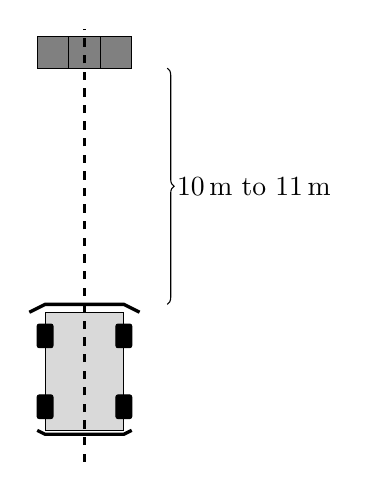
\begin{tikzpicture}
            \gokart{0}{0}{0}
        
            %Wall (three cubes)
            \draw[fill=gray] (-0.6,3) rectangle (-0.2,3.4);
            \draw[fill=gray] (-0.2,3) rectangle (0.2,3.4);
            \draw[fill=gray] (0.2,3) rectangle (0.6,3.4);
        
            %Dashed line from go-kart to wall
            \draw[dashed, thick] (0,-2) -- (0,3.5);

            \draw [decorate, decoration = {brace, raise=10pt}] (0.7,3) -- (0.7, 0) node[pos=0.5,right=10pt,black]{\SIrange{10}{11}{\meter}};
        \end{tikzpicture}
    %}
    \caption{Test scenario}
    \label{fig:test_scenario}
\end{figure}
The experimental setup consists of a Texas Instruments IWR6843AOPEVM development board, featuring the IWR6843AOP mmWave radar sensor, mounted at the front of a vehicle.  
The sensor provides point cloud data enriched with range, angle, and Doppler velocity information.  
This data forms the basis for the processing pipeline and enables the evaluation of radar odometry performance under realistic driving scenarios.  


\subsection{Sub-Tasks}

The research objective, together with the constraints of using a single radar sensor, implied several practical sub-tasks:  
\begin{itemize}
    \item Designing a pipeline to acquire and decode raw radar data.  
    \item Investigating suitable sensor configurations to balance field of view, update rate, and data density.  
    \item Implementing clustering methods to structure radar detections and isolate relevant features.  
    \item Integrating Doppler velocity information into the odometry estimation process.  
    \item Developing scan-to-scan registration using iterative closest point (ICP) optimization.  
    \item Employing submap aggregation to mitigate sparsity and improve stability.  
    \item Incorporating cluster-based tracking to filter dynamic objects from the ego-motion estimation.  
    \item Validating the complete system using recorded datasets and controlled driving experiments.  
\end{itemize}

As each sub-task builds upon the results of the previous one, the work followed an iterative and modular development approach, enabling gradual integration and continuous evaluation of the proposed system.  
\newpage

\section{IWR6843 Radar Interface and Configuration}
\label{sec:IWR6843 Radar Interface and Configuration}
The IWR6843AOPEVM development board from Texas Instruments features the IWR6843AOP, a high performance 4D mmWave FMCW radar sensor with Antenna On Package (AOP) design.
Although IWR6843AOP is intended for industrial applications and its complementary chip, AWR6843AOP, for automotive applications, IWR6843AOP was used in this project because it is available in the form of this development board and the two chips are identical in terms of their functionalities, only differing in compliance with automotive  industry \cite{iwr_awr_diff}.
Its small physical size, due to its AOP design, makes it an optimal choice for the desired mounting position, the go-kart's steering column.
\begin{figure}[!htbp]
    \centering
    \includegraphics[width=0.7\linewidth]{images/iwr6843aopevm-angled.png}
    \caption{IWR6843AOP sensor}
    \label{fig:IWR6843AOP sensor}
\end{figure}
\par
The IWR6843AOP radar sensor operates within the frequency range of \SIrange{60}{64}{\giga\hertz} and integrates 4 receive (RX) and 3 transmit (TX) antennas, radio frequency (RF) front-end stages, analog signal processing, and digital signal processing (DSP).
It offers a wide range of communication interfaces including SPI, I2C, CAN-FD, UART and LVDS for raw data access and an Arm Cortex-R4F microcontroller for user-applications \cite{dev_board_page}.
\begin{figure}[!htbp]
    \centering
    \includegraphics[width=1.0\linewidth]{images/blockdiagram.png}
    \caption{IWR6843AOP internal Block Diagram}
    \label{fig:IWR6843AOP_internal}
\end{figure}
\FloatBarrier\noindent
Texas Instruments offers various demo applications for the development board that utilize the internal microcontroller for showcasing the radar sensor's capabilities in different specialized scenarios.
It was found out that most of them only use the radar sensor itself only for obtaining a point cloud, which points include spatial information in form of $x,y,z$ coordinates and a radial speed information (the prior mentioned four dimensions of the sensor).
Application-specific processing of the point cloud itself is executed on an external computation device.
\par
The main demo application ("mmWave SDK demo") allows a versatile customization of the radar sensor's operating parameters and its discrimination capabilities while outputting the point cloud via its UART interface, accessible via the on-board USB to UART converter.
Although the demo seems to be intended to be used only for demonstration purposes, many projects based on Texas Instruments' mmWave radar sensors utilize it, because it poses a generic solution for obtaining (close to) real-time point cloud data from the sensor without prior development of a custom user-application for the radar sensor's internal microcontroller.
This setup was therefore chosen for supplying the emergency braking system with data.

\subsection{Utilizing the mmWave SDK demo}
The "mmWave SDK demo" was developed by Texas Instruments for showcasing the abilities of their mmWave radar sensors.
It consists of the radar sensor itself, supplying close to real-time point cloud data and an online tool for visualization of the raw output data and for the creation of a sequence of commands used for configuration of the radar sensor's operating parameters and output \cite{mmwave_demo_doc}.
Due to the demo's simple structure and the radar sensor's generic output, the online application can be replaced by a custom application replicating the online tool's behavior for making use of the data.
\par
In the demo application, the radar sensor opens two UART connections.
One connection is bidirectional at a lower speed of \SI{115200}{\baud} which is used to configure the radar sensor by sending the previously mentioned sequence of commands. 
The second connection is unidirectional, from the radar sensor to the receiver, at a higher speed of \SI{921600}{\baud} and is used for outputting a constant data stream after the radar sensor received its configuration and a start command.
As the data packets are encoded in a proprietary format and therefore need to be parsed prior to further processing, a custom software module was written in C++ and later ported to Python.
The module handles the radar sensor's setup by sending a configuration file containing the sequence of initialization commands and the cyclic parsing of the encoded data packets.
The sequence of commands was generated with Texas Instruments' online tool, as it provided graphical feedback while making the necessary compromises involved in setting up the radar sensor's operating parameters.

\subsection{Sensor Data Output Format}
As the data packets, containing the individual frames, are encoded in a proprietary format, they need to be parsed to allow for further processing.
Each frame starts with a frame header and contains a number of TLVs (Type, Length, Value) in which the actual payload data is stored\cite{mmwave_demo_doc}.
\begin{figure}[!htbp]
    \centering
    \includegraphics[width=0.4\linewidth]{images/UARTFrame.png}
    \caption{Frame structure. From \cite{mmwave_demo_output}.}
    \label{fig:UART data output format}
\end{figure}
\FloatBarrier\noindent
The frame's header has a total length of \SI{40}{\byte} and starts with a fixed magic word that denotes the start of each frame.
It also provides several other information in addition to the total packet length in bytes which is used to find the frame's end:
\begin{itemize}
    \item Magic Word: This value indicates the start of a new header, meaning that it can be used as a starting point for processing each frame.
    \item Total Packet Length: Total number of bytes in the frame (including the header) which can be used to calculate the frame's end.
    \item Platform: Indicates the device type and can be used for validating the radar sensor type. In the case of the device used for this project (IWR6843AOP) the expected value is "$0xA6843$".
    \item Number of TLVs: Total number of TLV's that exist in that specific frame.
\end{itemize}
\begin{figure}[!htbp]
    \centering
    \includegraphics[width=1.0\linewidth]{images/FrameFormatHeader.png}
    \caption{Frame header format. From \cite{mmwave_demo_output}.}
    \label{fig:Frame header format}
\end{figure}
\FloatBarrier\noindent
The frame contains one or more TLVs after its header.
Each TLV has a header itself in which it specifies its length and which type of data (point cloud, doppler heatmaps, statistics, ...) is contained inside.
Each TLV type needs to be decoded differently, as it represents a different type of data.
\begin{figure}[!htbp]
    \centering
    \includegraphics[width=0.95\linewidth]{images/TLVHeader.png}
    \caption{TLV header format. From \cite{mmwave_demo_output}.}
    \label{fig:TLV header format}
\end{figure}
\FloatBarrier

\subsection{Sensor Tuning}
As some operating parameters influence each other, their selection must be done carefully while observing the influence of the trade-offs involved.
This could be referred to as "sensor tuning" and is a critical step because it directly impacts the system's accuracy and performance.
\begin{comment}
Proper sensor tuning is critical because it directly impacts the accuracy and performance of the self-speed estimation, including the precision of the radial velocity and distance measurements derived from the returned radar waves.

Before initiating the sensor setup, it is crucial to identify the key parameters that will be monitored and adjusted. These parameters determine which aspects of the sensor's configuration need modification and help define the target performance criteria. Examples of these parameters include:
\end{comment}
The following operating parameters can be tuned:
\begin{itemize}
    \item Frame rate
    \item Range resolution
    \item Maximum unambigious range
    \item Maximum radial velocity
    \item Radial velocity resolution
\end{itemize}

Tuning these operating parameters introduces trade-offs by influencing each other in the following ways:
\begin{table}[h]
    \centering
    \resizebox{\columnwidth}{!}{%
    \begin{tabular}{|l|l|p{3.5cm}|p{3.5cm}|p{3.5cm}|}
        \hline
        \textbf{Tuning Parameter} & \textbf{Effect on Performance} & \textbf{Related HW Block} & \textbf{Trade-Off} \\
        \hline
        Frame Rate & Higher FPS = faster updates but more processing load & C674x DSP, Radar Data Memory & Higher FPS reduces maximum range \\
        \hline
        Range Resolution & Higher resolution = better object separation & ADC, 1D FFT (Range FFT) & Higher resolution reduces max range \\
        \hline
        Maximum Range & Determines farthest detectable object & RF Front-End, PA, LNA, ADC & Higher range lowers resolution \\
        \hline
        Radial Velocity Resolution & Improves speed accuracy & DSP, 2D FFT (Doppler FFT) & Higher resolution requires more chirps \\
        \hline
        Maximum Radial Velocity & Detects fast-moving objects & Chirp rate, TX Antennas, 2D FFT & Higher max velocity reduces resolution \\
        \hline
        %% [24/03/2025] Leander: Commented out because RCS depends on the target can not be tuned; is only used as a reference for calculating the range and stuff like this
        %Radar Cross Section (RCS) & Controls detection sensitivity based on object reflectivity & RF Front-End, LNA, ADC, DSP Filtering & Higher RCS increases range but may include unwanted reflections; Lower RCS improves accuracy but may miss small objects \\
        %\hline
    \end{tabular}%
    }
    \caption{Radar System Tuning Parameters and Trade-offs}
    \label{tab:mmWave_Sensor_Parameters}
\end{table}
The resulting overall accuracy of the velocity and distance measurements is again dependent on these operating parameters:
\begin{itemize}
    \item Radial velocity accuracy: A fine balance between velocity resolution and frame rate must be maintained to ensure precise doppler shift measurements. Lower resolution results in rounded velocity values, while an excessively high frame rate may introduce computational bottlenecks.
    \item Distance accuracy: Optimizing range resolution and maximum range ensures that detected objects are positioned accurately within the environment. Increasing range often sacrifices resolution, leading to potential inaccuracies in close-range detections.
    \item Signal Processing Considerations: The FFT calculation parameters directly affect both range and doppler calculations, influencing the ability to distinguish between objects and detect small velocity variations.
\end{itemize}
This shows that finding exact values for the operation parameters by adjusting them while carefully watching their influences is crucial and heavily dependent on the particular application.
The test scenario required an unambigious range of at least \SI{10}{\meter} and a maximum radial velocity of \SI{10}{\meter\per\second} due to its boundary conditions, together with the desire of the highest possible resolution of the radial velocity to ensure a reliable operation of the radar-based self-speed estimation.
Tuning yieled a configuration with the following operating parameters:
\begin{itemize}
    \item Frame rate: \SI{30}{\frame\per\second}
    \item Range resolution: \SI{0.178}{\meter}
    \item Maximum unambigious range: \SI{18.22}{\meter}
    \item Maximum radial velocity: \SI{10.24}{\meter\per\second}
    \item Radial velocity resolution: \SI{0.16}{\meter\per\second}
\end{itemize}

Tuning and choosing the sensor's parameters carefully is extremely important as it defines the accuracy of 
therefore influences the reliability of the entire radar system.
Fine-tuning these settings ensures that the sensor operates optimally, enabling more precise self-speed estimation and overall system performance.
The accuracy of radial speed estimation and distance measurements depends directly on the tuning of these parameters. A poorly configured sensor can result in erroneous velocity estimations, unreliable object detection, or excessive noise in Doppler measurements. An example of the influence of the selection of the correct parameters on the output point cloud of the radar sensor can be found in Fig.~\ref{fig:IWR6843AOP Calibration example2 for the sensor}.

\begin{figure}[!htbp]
    \centering
    \includegraphics[width=1.0\linewidth]{images/calib_ex.png}
    \caption{Output of the IWR6843AOP prior sensor tuning.}
    \label{fig:IWR6843AOP Calibration example for the sensor}
\end{figure}

\begin{figure}[!htbp]
    \centering
    \includegraphics[width=1.0\linewidth]{images/calib_ex2.png}
    \caption{Output of the IWR6843AOP after sensor tuning.}
    \label{fig:IWR6843AOP Calibration example2 for the sensor}
\end{figure}

\FloatBarrier

\section{Pipeline Implementation: Modules Implemented and Mathematical Explanation}
\label{sec:Mathematical Models and Algorithms for Radar-Based Object Detection}

To reliably interpret radar sensor data for static object detection and ego-motion estimation, a modular processing pipeline was developed. 
This pipeline supports both single-radar and dual-radar configurations, in both cases the inclusion of an Inertial Measurement Unit (IMU) is needed to compensate for rotational motion of the platform. 
The modular design allows adaptation to different vehicle setups and deployment conditions.

\subsection*{Sensor Data Preprocessing}
In the preprocessing of the radar data, there are two scenarios that were implemented for this project, the single-radar setup and the dual-radar setup with IMU integration.
In both radar setups, radar data is received over UART in the form of raw frames containing point cloud information. 
Each point includes its spatial coordinates $(x, y, z)$, radial velocity $v_r$, side-point info; this information comes with signal-to-noise ratio (SNR) and noise ration (dB) values that indicate the quality of each detection and range profile data.

The raw bytes are decoded \cite{understanding_uart} and structured into frame objects, which are then passed through a Physical Transformation module. 
This step converts from the sensor frame coordinates into the vehicle local frame, accounting for radar mounting position and orientation. 
This can be consider a rigid body transformation involving rotation and translation matrices.
However is really important that this process of rigid transformation is done, as the data that we obtain from the sensor does not know where it is in the vehicle, creating a missalignment between the radar data and the vehicle frame of reference.

\subsubsection*{Dual-Radar Configuration}
In the dual-radar configuration, two front-facing sensors are mounted symmetrically on the left and right sides of the vehicle, providing overlapping fields of view. 
This arrangement expands the effective coverage and reduces blind spots, offering a broader perception range compared to a single-radar setup.  

The use of two radars requires careful calibration to avoid interference effects, such as ghost detections or false targets, and to ensure consistent alignment of their outputs.  
When properly tuned, the dual-radar configuration produces a denser and more reliable point cloud, serving as a stronger foundation for subsequent stages of the odometry pipeline.

\subsection*{Frame Aggregation}
Radar point clouds are naturally sparse, especially at longer ranges. 
To improve stability and robustness, consecutive frames are aggregated into a local submap. 
This approach increases point density, reduces the effect of random noise, and provides a richer structure for downstream tasks such as clustering and alignment. 
The aggregation is performed after IMU-based alignment, ensuring that the fused frames are geometrically consistent. 

\subsection*{Filtering and Self-Speed Estimation}
Once points are aggregated and aligned, the pipeline performs filtering in two stages:

\begin{itemize}
    \item \textbf{Coordinate and SNR Filtering:} Removes points outside valid spatial boundaries or below a configurable SNR threshold.
    \item \textbf{Velocity-based Filtering:} Applies a Doppler threshold to remove points with radial velocities below or above predefined limits. This eliminates static clutter and extreme outliers, leaving only detections within the valid motion range.
\end{itemize}

From the remaining points, the vehicle self-speed is estimated using the Doppler measurements. 
A Kalman filter is then applied to smooth fluctuations and provide a stable velocity estimate, which is reused in subsequent stages of the odometry pipeline.

\subsection*{Clustering and Outlier Rejection}
The filtered detections are organized into clusters to provide structure to the radar scene. 
A two-stage clustering strategy is employed to gradually refine the set of candidate targets:  

\begin{itemize}
    \item \textbf{Stage 1 – Permissive Clustering:} A loose grouping is applied using the DBSCAN algorithm, which is well-suited for radar point clouds since it does not require the number of clusters to be specified in advance and can naturally separate sparse detections. 
    At this stage, the parameters are set permissively, allowing loosely associated points to be grouped into preliminary clusters so that potential targets are not discarded prematurely.  
    \item \textbf{Stage 2 – Strict Clustering:} The preliminary clusters are reprocessed with stricter DBSCAN parameters, enforcing tighter geometric proximity between points. 
    This refinement step eliminates loosely connected points and isolates only the detections that are spatially consistent, resulting in compact and reliable target clusters.  
\end{itemize}

This hierarchical approach ensures that targets are first captured broadly and then refined to retain only geometrically close detections, which are more suitable for downstream odometry estimation.  
Additionally, RANSAC-based outlier rejection is performed prior to clustering, further reducing the influence of inconsistent or spurious points on the cluster formation.  

DBSCAN's ability to handle varying cluster shapes, adapt to density variations, and explicitly label noise points makes it particularly advantageous in radar applications, where detections are inherently sparse, noisy, and often non-uniformly distributed.

\subsection*{ICP Alignment and Ego-Motion Estimation}
The final stage of the pipeline estimates vehicle motion by applying the Iterative Closest Point (ICP) algorithm for frame-to-frame alignment. 
ICP iteratively minimizes the distance between corresponding points across consecutive frames, computing the rigid-body transformation that best aligns them.  

In this project, ICP was applied under two distinct configurations for analysis:  

\begin{itemize}
    \item \textbf{Global ICP:} The entire aggregated point cloud from consecutive frames is used for alignment. 
    This approach provides a direct estimate of ego-motion but is sensitive to outliers and dynamic objects present in the scene.  

    \item \textbf{Cluster-based ICP:} Instead of aligning full point clouds, ICP is applied selectively on clusters identified as static targets. 
    By focusing on geometrically consistent regions, this method looks to improve robustness against moving objects and to enhance the stability of the motion estimate.  
\end{itemize}

The outcome of ICP is a rigid transformation that represents the vehicle's ego-motion between frames, serving as the foundation for radar-based odometry.

\begin{figure*}[!htbp]
    \centering
    \resizebox{\textwidth}{!}{%
        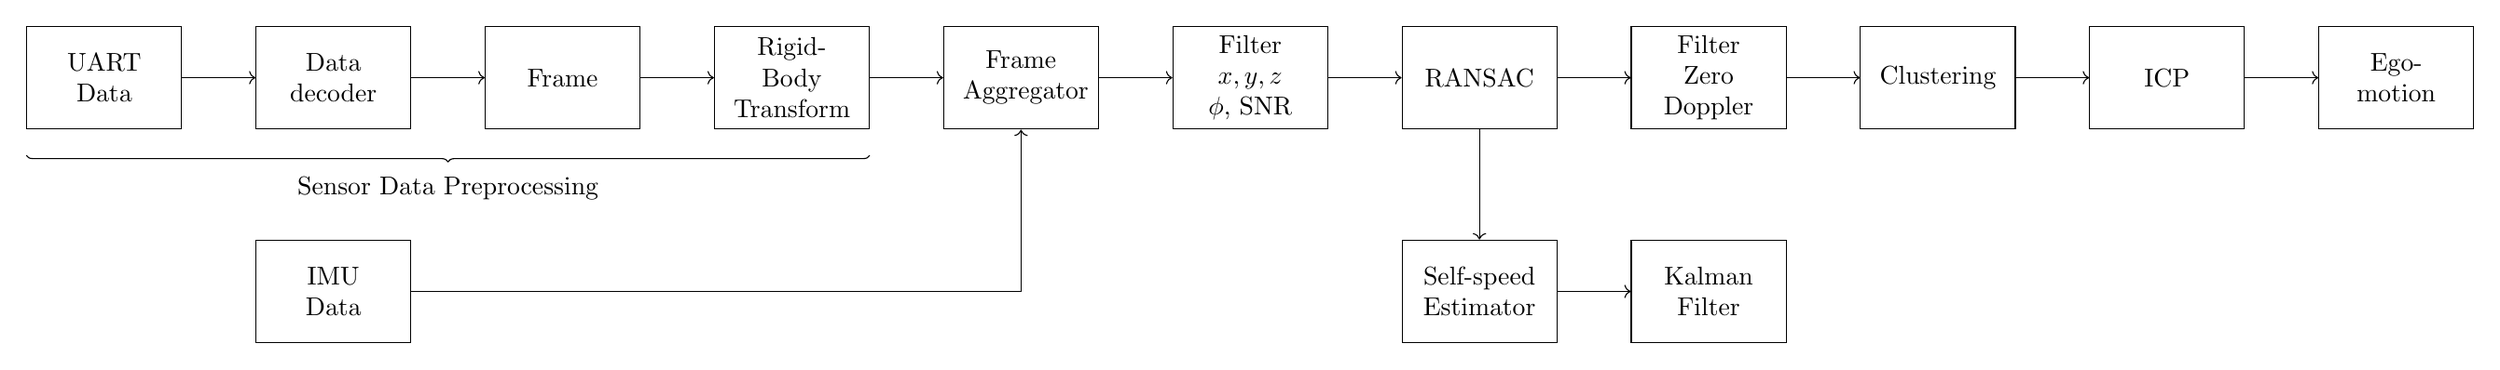
\begin{tikzpicture}
            % Block style
            \tikzstyle{block} = [rectangle, draw, text width=4.5em, text centered, minimum width=6em, minimum height=4em]

            % Upper row
            \node[block] (uart) {UART\\Data};
            \node[block, right=of uart] (decoder) {Data decoder};
            \node[block, right=of decoder] (frames) {Frame};
            \node[block, right=of frames] (transform) {Rigid-Body\\Transform};
            \node[block, right=of transform] (frame_aggr) {Frame\\Aggregator};
            \node[block, right=of frame_aggr] (coord_filter) {Filter\\$x,y,z$\\$\phi$, SNR};
            \node[block, right=of coord_filter] (ransac) {RANSAC};
            \node[block, right=of ransac] (doppler_filter) {Filter\\Zero Doppler};
            \node[block, right=of doppler_filter] (clustering) {Clustering};
            \node[block, right=of clustering] (icp) {ICP};
            \node[block, right=of icp] (ego) {Ego-motion};

            % IMU and self-speed estimator (below RANSAC)
            \node[block, below=1.5cm of decoder] (imu) {IMU\\Data};
            \node[block, below=1.5cm of ransac] (self_speed_estim) {Self-speed Estimator};
            \node[block, right=of self_speed_estim] (self_speed_kalman) {Kalman Filter};

            % Connections
            \draw[->] (uart) -- (decoder);
            \draw[->] (decoder) -- (frames);
            \draw[->] (frames) -- (transform);
            \draw[->] (transform) -- (frame_aggr);
            \draw[->] (imu.east) -| ([yshift=-1.5em]frame_aggr.south) -| (frame_aggr.south);

            \draw[->] (frame_aggr) -- (coord_filter);
            \draw[->] (coord_filter) -- (ransac);
            \draw[->] (ransac) -- (doppler_filter);
            \draw[->] (doppler_filter) -- (clustering);
            \draw[->] (clustering) -- (icp);
            \draw[->] (icp) -- (ego);

            \draw[->] (ransac.south) -- (self_speed_estim.north);
            \draw[->] (self_speed_estim) -- (self_speed_kalman);

            % Bottom brace for preprocessing
            \draw [decorate, decoration = {brace, mirror, raise=10pt}]
                (uart.south west) -- (transform.south east)
                node[pos=0.5,below=15pt,black]{Sensor Data Preprocessing};
        \end{tikzpicture}
    }
    \caption{Single Radar Pipeline}
    \label{fig:single_radar_pipeline}
\end{figure*}

\begin{figure*}[!htbp]
    \centering
    \resizebox{\textwidth}{!}{%
        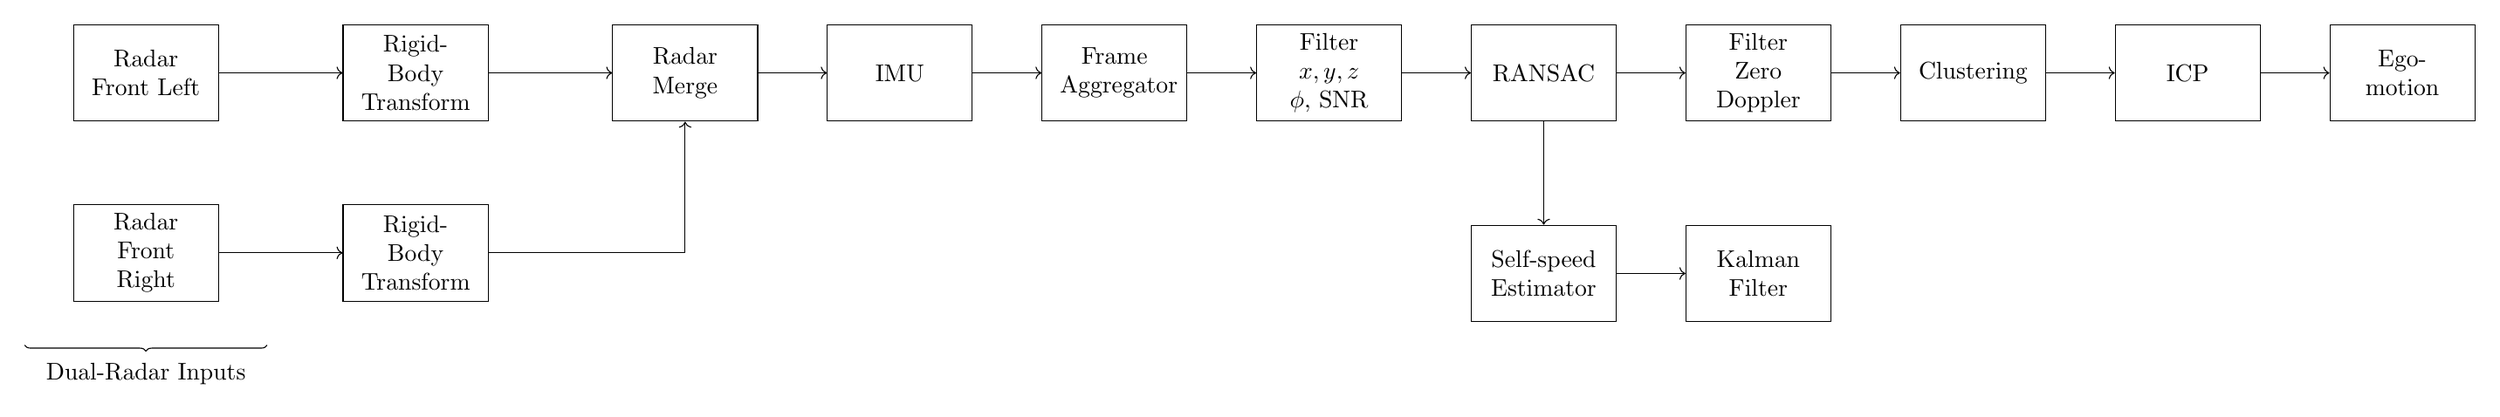
\begin{tikzpicture}
            % Block style
            \tikzstyle{block} = [rectangle, draw, text width=4.5em, text centered, minimum width=6em, minimum height=4em]

            % Input branches
            \node[block] (radar1) {Radar\\Front Left};
            \node[block, below=1.2cm of radar1] (radar2) {Radar\\Front Right};

            % Physical transformation
            \node[block, right=1.8cm of radar1] (transform1) {Rigid-Body\\Transform};
            \node[block, below=1.2cm of transform1] (transform2) {Rigid-Body\\Transform};

            % Merge and processing
            \node[block, right=1.8cm of transform1] (merge) {Radar Merge};
            \node[block, right=of merge] (imu) {IMU};
            \node[block, right=of imu] (frame_aggr) {Frame\\Aggregator};
            \node[block, right=of frame_aggr] (coord_filter) {Filter\\$x,y,z$\\$\phi$, SNR};
            \node[block, right=of coord_filter] (ransac) {RANSAC};
            \node[block, right=of ransac] (doppler_filter) {Filter\\Zero Doppler};
            \node[block, right=of doppler_filter] (clustering) {Clustering};
            \node[block, right=of clustering] (icp) {ICP};
            \node[block, right=of icp] (ego) {Ego-motion};

            % Self-speed estimator (below RANSAC)
            \node[block, below=1.5cm of ransac] (self_speed_estim) {Self-speed Estimator};
            \node[block, right=of self_speed_estim] (self_speed_kalman) {Kalman Filter};

            % Connections
            \draw[->] (radar1) -- (transform1);
            \draw[->] (radar2) -- (transform2);
            \draw[->] (transform1) -- (merge);
            \draw[->] (transform2) -| (merge);
            \draw[->] (merge) -- (imu);
            \draw[->] (imu) -- (frame_aggr);
            \draw[->] (frame_aggr) -- (coord_filter);
            \draw[->] (coord_filter) -- (ransac);
            \draw[->] (ransac) -- (doppler_filter);
            \draw[->] (doppler_filter) -- (clustering);
            \draw[->] (clustering) -- (icp);
            \draw[->] (icp) -- (ego);

            \draw[->] (ransac.south) -- (self_speed_estim.north);
            \draw[->] (self_speed_estim) -- (self_speed_kalman);

            % Bottom brace under radar2
            \draw [decorate, decoration = {brace, mirror, raise=8pt}] 
                ([xshift=-2em,yshift=-1em]radar2.south west) -- 
                ([xshift=2em,yshift=-1em]radar2.south east)
                node[midway, below=12pt] {Dual-Radar Inputs};
        \end{tikzpicture}
    }
    \caption{Dual Radar Pipeline}
    \label{fig:dual_radar_pipeline}
\end{figure*}



\FloatBarrier\noindent
\input{section/06FrameAggregator}
\subsection{"$x,y,z,\phi,SNR$" Filter}
The point cloud's points are passed through a first static filtering stage to remove points caused by noise, clutter or targets outside of the area of interest before being used for further processing.
This static filtering stage consists of four different filters, filtering out points by different attributes:
\begin{enumerate}
    \item Filtering by $SNR$: All points with a $SNR$ lower than \SI{12}{\deci\bel} are filtered out to remove points with a low signal and those that might be caused by noise or clutter.
    \item Filtering by $z$ coordinate: All points below a $z$ value of \SI{0}{\meter} and above \SI{2}{\meter} are filtered out to remove points caused by the ground or the ceiling.
    \item Filtering by $y$ coordinate: All points below a $y$ value of \SI{0.3}{\meter} are filtered out to remove points created by the driver's feet.
    \item Filtering by $\phi$: All points with an azimuth bigger than \SI{85}{\degree} are filtered out to remove points that are outside the area of interest.
\end{enumerate}
\textit{Note: The origin of the points' coordinate system is the sensor itself, so a coordinate of $(\SI{0}{\meter},\SI{0}{\meter},\SI{0}{\meter})$ is essentially at the sensor's mounting position and therefore approx. \SI{0.3}{\meter} above the ground.}
\par
As the static filtering stage only keeps points which are relevant in terms of there spatial position and $SNR$ for the following stages, it effectively decreases the computation time of each frame and prevents the following stages from processing invalid data.
The filtered point cloud is then passed to the next stages, the self-speed estimator and the dynamic filtering stage.

\begin{figure}[!htbp]
\centering
\begin{subfigure}{0.24\textwidth}
  \centering
  \includegraphics[width=\textwidth]{images/No_filter.png}
  \caption{Input}
\end{subfigure}
\begin{subfigure}{0.24\textwidth}
  \centering
  \includegraphics[width=\textwidth]{images/filter.png}
  \caption{Output}
\end{subfigure}
\caption{Example visualization of the input and output when filtering by the value of the $z$ coordinate.}
\label{fig:static_filter_z_example}
\end{figure}
\FloatBarrier\noindent

%% [20/03/2025] Leander: Rework done, commentend out bc. probably not needed anymore
%% ---------------------------------------
\begin{comment}
(effectively the radar sensor's mounting height as the coordinate's origin is at the sensor; approx. \SI{30}{\centi\meter} above ground) and \SI{2}{} 
Physical filtering further refines the data, this by removing points that can be considered as environmental noise or clutter, points outside the sensor’s effective monitoring area, or points whose radar cross-section (RCS) values fall below a predetermined threshold.
By mentioning the sensor effective monitoring area it is considered as area that the sensor will gather the information, process it and then give it as a result. But we might not be interested in all of this information.

\begin{figure}[!htbp]
\centering
\begin{subfigure}{0.24\textwidth}
  \centering
  \includegraphics[width=\textwidth]{images/filter.png}
\end{subfigure}
\begin{subfigure}{0.24\textwidth}
  \centering
  \includegraphics[width=\textwidth]{images/No_filter.png}
\end{subfigure}
\caption{The physical filters help us consider only information that may be caught by the sensor, but is of no use for us.}
\label{fig:remote_controller_components}
\end{figure}

For the project application and sensor location, it is considered that a Z-axis filter it is needed. As it will add more points that we will process if we don't discard them for the processing of the point-cloud.

This same concept may apply for other physical values of the point-cloud data, this being radial speed. If a point with a radial speed that is considered just ridiculous, then we add that point to the discarded data.
\end{comment}
\input{section/08SelfSpeedEstimation}
\input{section/09Kalman}
\input{section/10VeVsSelfspeed}

\subsection{Clustering}
Clustering is a fundamental technique used to group similar data points based on their characteristics. It is particularly useful in sensor data analysis for automotive applications, enabling the effective detection and tracking of objects such as vehicles, obstacles, and pedestrians.
\par
Among various clustering algorithms available, DBSCAN (Density-Based Spatial Clustering of Applications with Noise) stands out due to its ability to automatically detect clusters of varying shapes and sizes (see \cite{geeksforgeeks_dbscan}), and to effectively identify and manage noise or outliers. Unlike centroid-based methods such as K-means, which require specifying the number of clusters in advance and struggle with irregularly shaped data, DBSCAN identifies clusters based on the density distribution of data points. Additionally, hierarchical methods like agglomerative clustering, although flexible, tend to be sensitive to noise and computationally expensive for large datasets.

\begin{table}[htbp]
\centering
\resizebox{\columnwidth}{!}{%
\begin{tabular}{|l|l|p{3.5cm}|p{3.5cm}|p{3.5cm}|}
\hline
\textbf{Algorithm} & \textbf{Type} & \textbf{Strengths} & \textbf{Weaknesses} & \textbf{Best Use Case} \\ \hline
DBSCAN & Density-Based & \begin{itemize}
    \item Automatically detects clusters of \textbf{different shapes and sizes}
    \item Identifies \textbf{outliers (noise points)}
\end{itemize} & \begin{itemize}
    \item Computationally expensive for \textbf{large datasets}
\end{itemize} & Radar object detection with noise filtering \\ \hline
K-Means & Centroid-Based & \begin{itemize}
    \item Fast and efficient for \textbf{large datasets}
\end{itemize} & \begin{itemize}
    \item Requires a \textbf{fixed number of clusters (K)}
    \item Struggles with \textbf{irregularly shaped clusters}
\end{itemize} & Segmenting structured radar data with known object counts \\ \hline
Agglomerative & Hierarchical & \begin{itemize}
    \item Does not require specifying number of clusters
    \item Can be modified to detect \textbf{hierarchical structures}
\end{itemize} & \begin{itemize}
    \item Can be \textbf{sensitive to noise}
    \item Computationally expensive for \textbf{large datasets}
\end{itemize} & Grouping similar radar signatures in post-processing \\ \hline
\end{tabular}%
}
\caption{Comparison of Clustering Algorithms}
\label{tab:clustering_algorithms}
\end{table}

For this project, DBSCAN's strengths align closely with the requirements of radar object detection, where the number of detected objects can change dynamically and the presence of noise is common. DBSCAN's capability to handle varying densities and noisy data makes it the optimal choice for accurately and efficiently analyzing real-time radar sensor data in automotive applications.

However, this is insufficient to fully meet the requirements of object detection. It is acknowledged that DBSCAN is among the most efficacious and straightforward instruments available for achieving this objective. However, it is important to note that the sizes of the objects under observation can vary significantly from one frame to the next, and the presence of noise can introduce additional variability. To address these challenges, a two-stage clustering approach was chosen, utilizing DBSCAN as a filter and a clustering algorithm.
The first stage that acts as a filter with DBSCAN parameterized by an Epsilon of \SI{2}{\meter} and a minimum number of samples to specify a core point of 2.
The justification for using it as a filter is that, at first, a broad or permissive set of parameters is applied, making it easier to filter out points or data that are considered as noise. This is not due to the presence of "real" noise; rather, it is owing to a lack of the required amount of points to qualify as an object.
This principle is represented in the next figure:
\begin{figure}[!htbp]
    \centering
    \includegraphics[width=1.0\linewidth]{images/clustering.png}
    \caption{First clustering stage}
    \label{fig: First clustering stage}
\end{figure}
\FloatBarrier\noindent
It can be seen that there are three points that are not included in the clusters and seem to be outliers.
These points might belong to an object, but most likely they are caused by clutter or noise.
As they are not included in clusters after first stage, they are discarded and only the points that are included in clusters are passed to the second stage.
\par
The second stage utilizes DBSCAN with a finer set of parameters.
In this stage, Epsilon was chosen to be equal to \SI{1}{\meter} and the minimum number of samples to specify a core point was set to 4.
This results in finer clusters, preventing objects which are close to each other to be recognized as one single cluster.
The clusters are then passed to the brake controller for final object detection and handling of approaching targets.
\subsection{Brake Controller}

A brake controller is a crucial component in autonomous and assisted driving systems, enabling vehicles to respond intelligently to detected obstacles or hazards.
In this project, a simple yet effective braking mechanism was implemented using a linear controller that calculates a safe stopping distance based on the vehicle's current speed.
The controller assumes a linear relationship between speed and stopping distance, a reasonable approximation under controlled conditions and for the rather lightweight go-kart.
The controller's objective is to ensure that if the vehicle is approaching an obstacle inside an area of interest and potentially getting into contact with it, it activates the brake early enough to stop within a safe distance.
Here, the area of interest is a specified area in front of the go-kart encasing the space where an approaching stationary obstacle could become a hazard to the driver and vehicle.
As the distance which is required to stop the vehicle before getting into contact with the obstacle is proportional to the vehicle's speed, the length of the area of interest is coupled to it.
\par
The brake controller's logic is based on the following variables:
\begin{itemize}
    \item Stopping distance $d_{\text{stop}}(v_{\text{current}})$: Estimates how much distance the vehicle requires to come to a complete stop at the current speed, according to the vehicle specifications.
    \item Output signal $brake\_signal(d_{\text{stop}},d_{\text{target}})$: Generates a binary brake signal (0 or 1) based on whether the stopping distance exceeds the target distance. As the current brake controller simply considers if the brake should be applied or not.
\end{itemize}
The stopping distance is computed relative to a reference speed and stopping distance (default: 40~kph $\rightarrow$ 6~meters), allowing for linear scaling:
\[
d_{\text{stop}}(v_{\text{current}}) = \frac{v_{\text{current}}}{v_{\text{ref}}} \cdot d_{\text{ref}}
\]
If the required stopping distance is greater than or equal to the available distance (measured distance to a detected obstacle), the system triggers full braking:
\[
brake\_signal(d_{\text{stop}},d_{\text{target}}) =
\begin{cases}
1 & \text{if } d_{\text{target}} \leq d_{\text{stop}} \\
0 & \text{otherwise}
\end{cases}
\]

\begin{figure}[!htbp]
    \centering
    \includegraphics[width=0.8\linewidth]{images/brakeSignal.png}
    \caption{Braking decision based on stopping distance estimation.}
    \label{fig:braking_logic}
\end{figure}
This straightforward logic allows the controller to make quick decisions in real time, helping the vehicle to react safely to moving and stationary objects, detected by the radar.
Although the system is designed to be cautious because it only switches between braking and not braking, it could be improved later by adding smoother braking or more advanced features like adaptive cruise control.
The controller plays a key role in the interaction between detection (from the radar sensor's output data and the processing pipeline) and actuation (braking), forming the basis for a closed-loop safety mechanism.
\section{Summary and Outlook}

Insert conclusion here
%\section{WIP - Storing TikZ graphics}

\begin{figure}[!htbp]
    \centering
    \resizebox{0.48\textwidth}{!}{
        \begin{tikzpicture}
            % Block styles
            \tikzstyle{block} = [rectangle, draw, text width=4.5em, text centered, minimum width=6em, minimum height=4em]
            \tikzstyle{block_dashed} = [rectangle, draw, text width=2em, text centered, minimum width=4em, minimum height=4em, dashed]
            % Input and output
            \node[block, right=of antenna, minimum width=4em, minimum height=4em] (frames) {Frames};
            \node[block, right=of frames] (frame_aggr) {Frame\\Aggregator};
            \node[block, right=of frame_aggr] (coord_filter) {Filter\\$x,y,z$\\$\phi,SNR$};
            \node[block, right=of coord_filter] (self_speed_estim) {Self-speed Estimator};
            \node[block, right=of self_speed_estim] (self_speed_kalman) {Kalman Filter};
            \node[block, below=of self_speed_estim] (ve_speed_calc) {Calculation\\of $v_{e}$};
            \node[block, right=of ve_speed_calc] (ve_filter) {Filter\\$v_{e}$ vs. self-speed};
            \node[block, right=of ve_filter] (clustering) {Clustering};
            % Connections
            \draw[->] (frames) -- (frame_aggr); % Connection from antenna to RF amplifier
            \draw[->] (frame_aggr) -- (coord_filter);
            \draw[->] (coord_filter) -- (self_speed_estim);
            \draw[->] (coord_filter.south) |- (ve_speed_calc.west);
            \draw[->] (self_speed_estim) -- (self_speed_kalman);
            \draw[->] (self_speed_kalman) -- (ve_filter);
            \draw[->] (ve_speed_calc) -- (ve_filter);
            \draw[->] (ve_filter) -- (clustering);
        \end{tikzpicture}
    }
    \caption{Block diagram of the pipeline}
    \label{fig:block_diag_pipeline}
\end{figure}

\begin{figure}[!htbp]
    \centering
    \resizebox{0.48\textwidth}{!}{
        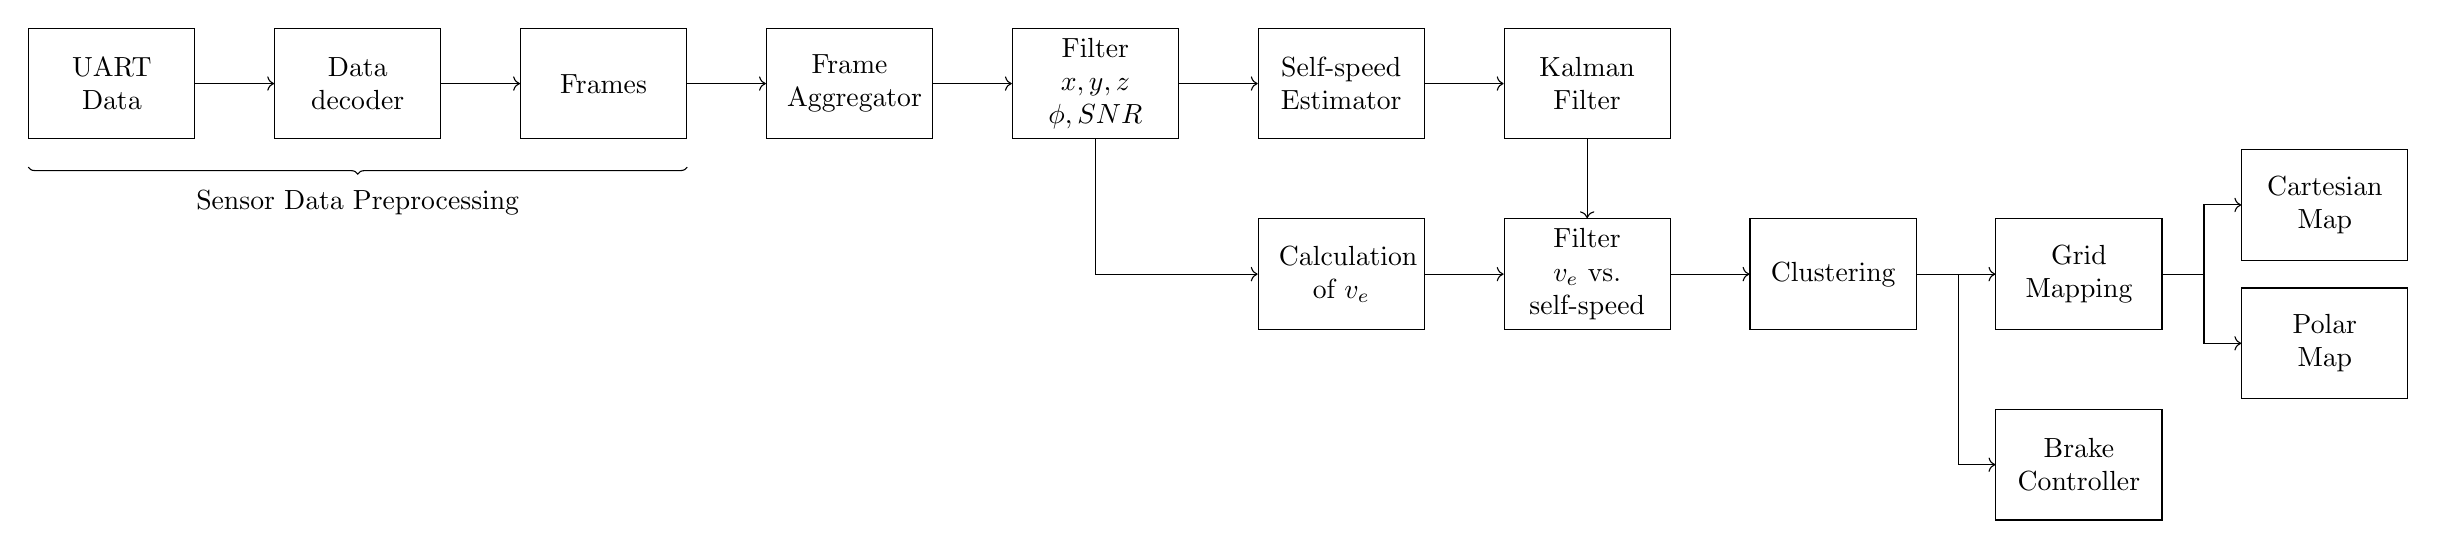
\begin{tikzpicture}
            % Block styles
            \tikzstyle{block} = [rectangle, draw, text width=4.5em, text centered, minimum width=6em, minimum height=4em]
            \tikzstyle{block_dashed} = [rectangle, draw, text width=2em, text centered, minimum width=4em, minimum height=4em, dashed]
            % Input and output
            \node[block] (uart) {UART\\Data};
            \node[block, right=of uart] (decoder) {Data decoder};
            \node[block, right=of decoder] (frames) {Frames};
            \node[block, right=of frames] (frame_aggr) {Frame\\Aggregator};
            \node[block, right=of frame_aggr] (coord_filter) {Filter\\$x,y,z$\\$\phi,SNR$};
            \node[block, right=of coord_filter] (self_speed_estim) {Self-speed Estimator};
            \node[block, right=of self_speed_estim] (self_speed_kalman) {Kalman Filter};
            \node[block, below=of self_speed_estim] (ve_speed_calc) {Calculation\\of $v_{e}$};
            \node[block, right=of ve_speed_calc] (ve_filter) {Filter\\$v_{e}$ vs. self-speed};
            \node[block, right=of ve_filter] (clustering) {Clustering};
            \node[block, right=of clustering] (grid_mapping) {Grid Mapping};
            \node[block, right=of grid_mapping.east, yshift=2.5em] (grid_cartesian) {Cartesian\\Map};
            \node[block, right=of grid_mapping.east, yshift=-2.5em] (grid_polar) {Polar\\Map};
            \node[block, below=of grid_mapping] (brake) {Brake\\Controller};
            % Connections
            \draw[->] (uart) -- (decoder);
            \draw[->] (decoder) -- (frames);
            \draw[->] (frames) -- (frame_aggr); % Connection from antenna to RF amplifier
            \draw[->] (frame_aggr) -- (coord_filter);
            \draw[->] (coord_filter) -- (self_speed_estim);
            \draw[->] (coord_filter.south) |- (ve_speed_calc.west);
            \draw[->] (self_speed_estim) -- (self_speed_kalman);
            \draw[->] (self_speed_kalman) -- (ve_filter);
            \draw[->] (ve_speed_calc) -- (ve_filter);
            \draw[->] (ve_filter) -- (clustering);

            \draw[-] (clustering.east) --++(1.5em, 0) coordinate (arrw_clustering);
            \draw[->] (arrw_clustering) -- (grid_mapping);
             \draw[->] (arrw_clustering) |- (brake);

            \draw[-] (grid_mapping.east) --++(1.5em, 0) coordinate (arrw_mapping_grids);
            \draw[->] (arrw_mapping_grids) |- (grid_cartesian.west);
            \draw[->] (arrw_mapping_grids) |- (grid_polar);

            \draw [decorate, decoration = {brace, mirror, raise=10pt}] (uart.south west) --  (frames.south east) node[pos=0.5,below=15pt,black]{Sensor Data Preprocessing};
        \end{tikzpicture}
    }
    \caption{Block diagram of the pipeline}
    \label{fig:block_diag_pipeline}
\end{figure}


\begin{figure}[!htbp]
    \centering
    \resizebox{0.48\textwidth}{!}{
        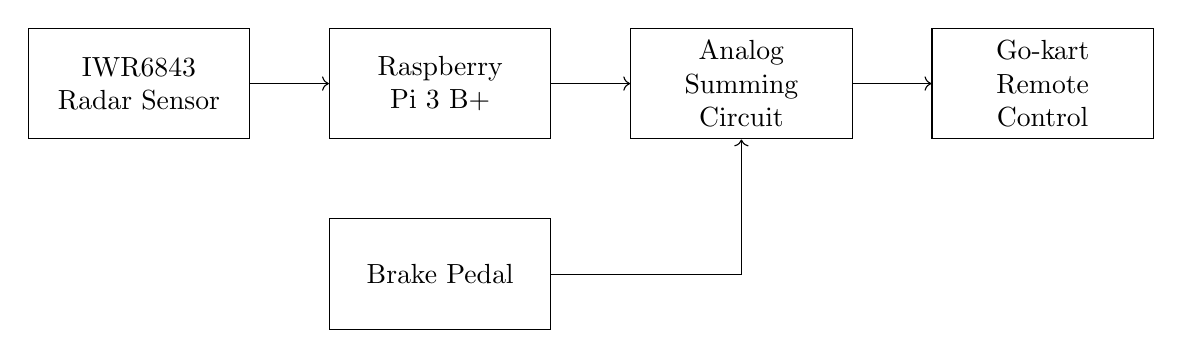
\begin{tikzpicture}
            % Block styles
            \tikzstyle{block} = [rectangle, draw, text width=6.5em, text centered, minimum width=8em, minimum height=4em]
            \tikzstyle{block_dashed} = [rectangle, draw, text width=2em, text centered, minimum width=4em, minimum height=4em, dashed]
            % Input and output
            \node[block] (radar) {IWR6843\\Radar Sensor};
            \node[block, right=of radar] (rpi) {Raspberry\\Pi 3 B+};
            \node[block, right=of rpi] (analog_summ) {Analog Summing\\Circuit};
            \node[block, below=of rpi] (brake_pedal) {Brake Pedal};
            \node[block, right=of analog_summ] (remote) {Go-kart\\Remote Control};
            % Connections
            \draw[->] (radar) -- (rpi);
            \draw[->] (rpi) -- (analog_summ);
            \draw[->] (brake_pedal) -| (analog_summ);
            \draw[->] (analog_summ) -- (remote);
        \end{tikzpicture}
    }
    \caption{Block diagram of the pipeline}
    \label{fig:block_diag_pipeline}
\end{figure}
\newpage

\begin{thebibliography}{00}

\bibitem{ninebot_product_page} Segway Inc., ``Ninebot Go-kart PRO product page'', 2025, Webpage. [Online]. Available: \url{https://de-de.segway.com/products/ninebot-gokart-pro}

\bibitem{iwr_awr_diff} Texas Instruments, ``IWR1642: difference between AWR and IWR parts'', 2025, Webpage. [Online]. Available: \url{https://e2e.ti.com/support/sensors-group/sensors/f/sensors-forum/742730/iwr1642-difference-between-awr-and-iwr-parts}

\bibitem{dev_board_page} Texas Instruments, ``IWR6843AOPEVM product page'', 2025, Webpage. [Online]. Available: \url{https://www.ti.com/tool/IWR6843AOPEVM}

\bibitem{mmwave_demo_doc} Texas Instruments, ``User's Guide mmWave Demo Visualizer,'' 2020, Online Document. [Online]. Available: \url{https://www.ti.com/lit/ug/swru529c/swru529c.pdf?ts=1742817596204}.

\bibitem{mmwave_demo_web} 
Texas Instruments, 
``mmWave Demo Visualizer'', 2025, Webpage. [Online]. Available: \url{https://dev.ti.com/gallery/view/mmwave/mmWave_Demo_Visualizer/ver/3.6.0/}

\bibitem{understanding_uart} Texas Instruments, ``Understanding UART Data Output Format'', 2025, Webpage. [Online]. Available: \url{https://dev.ti.com/tirex/content/radar_toolbox_2_20_00_05/docs/software_guides/Understanding_UART_Data_Output_Format.html}

\bibitem{mmwave_demo_output} Texas Instruments, ``mmWave Sensing Estimator'', 2025, Webpage. [Online]. Available: \url{https://dev.ti.com/gallery/view/mmwave/mmWaveSensingEstimator/ver/2.5.1/}

\bibitem{ninebot_protocol_github} ub4raf, ``Ninebot-PROTOCOL'', 2025, GitHub Repository. [Online]. Available: \url{https://github.com/ub4raf/Ninebot-PROTOCOL}

\bibitem{ninebot_protocol_scooterhacking} -, ``Ninebot ES Communicaton Protocol'', 2019, Webpage. [Online]. Available: \url{https://cloud.scooterhacking.org/release/nbdoc.pdf}

\bibitem{numpy_polyfit} -, ``numpy.polyfit documentation'', 2025, Webpage. [Online]. Available: \url{https://numpy.org/doc/stable/reference/generated/numpy.polyfit.html}

\bibitem{OccupancyGrid_Mapping_Automotive} Ç. Önen, A. Pandharipande, G. Joseph, and N. J. Myers, ``Occupancy Grid Mapping for Automotive Driving Exploiting Clustered Sparsity,'' \textit{IEEE Sensors Journal}, vol. 24, no. 7, pp. 9240-9250, 2024. [Online]. Available: \url{https://doi.org/10.1109/JSEN.2023.3342463}.

\bibitem{Odometry_radar_only}
D. Casado Herraez, M. Zeller, L. Chang, I. Vizzo, M. Heidingsfeld, and C. Stachniss, 
``Radar-Only Odometry and Mapping for Autonomous Vehicles,'' 
\textit{arXiv preprint}, 2023. [Online]. Available: \url{https://arxiv.org/abs/2305.12409}

\bibitem{EgoMotion_DopplerRadar}
S. R. Bhatt, B. S. Nadiger, R. Parthasarathy, and H. M. Shetty, 
``Instantaneous Ego-motion Estimation Using Doppler Radar,'' 
\textit{IEEE Sensors Letters}, vol. 7, no. 5, pp. 1–4, 2023. [Online]. Available: \url{https://doi.org/10.1109/LSENS.2023.3244030}

\bibitem{Multimodal_Offroad}
C. E. Beal, T. Williams, J. Pauli, M. Mukadam, and B. Boots, 
``Robust Off-Road Autonomy Using Multimodal Sensor Fusion,'' 
in \textit{Proc. of the Conference on Robot Learning (CoRL)}, 2023. [Online]. Available: \url{https://openreview.net/forum?id=kmiZqSgoAt}

\bibitem{HighSpeed_Estimation}
B. Sundaralingam, C. E. Beal, and B. Boots, 
``Robust High-Speed State Estimation for Off-Road Autonomous Vehicles,'' 
in \textit{Proc. of Robotics: Science and Systems (RSS)}, 2023. [Online]. Available: \url{https://openreview.net/forum?id=3JpFLY3ihix}


\bibitem{geeksforgeeks_dbscan}
GeeksforGeeks, 
\emph{DBSCAN Clustering in ML | Density Based Clustering}, 
2023. [Online]. Available: \url{https://www.geeksforgeeks.org/dbscan-clustering-in-ml-density-based-clustering/}. [Accessed: 19-Mar-2025].

\bibitem{mathworks_kalman}
MathWorks,
\textit{Understanding Kalman Filters, Part 3: Optimal State Estimator},
2017. Available at: \url{https://la.mathworks.com/videos/understanding-kalman-filters-part-3-optimal-state-estimator--1490710645421.html} (Accessed: March 23, 2025).

\bibitem{ti_radar_toolbox}
Texas Instruments, 
\textit{Radar Toolbox – mmWave Sensor Configuration and Demos}, 
2024. Available at: \url{https://dev.ti.com/tirex/explore/node?node=A__ADnbI7zK9bSRgZqeAxprvQ__radar_toolbox__1AslXXD__2.20.00.05} (Accessed: March 23, 2025).

\bibitem{mti710_manual}  
Movella (Xsens),  
\textit{MTi User Manual},  
2023. [Online]. Available: \url{https://www.xsens.com/hubfs/Downloads/usermanual/MTi_usermanual.pdf}. [Accessed: 26-Sep-2025].  

\bibitem{xsens_repo}  
Scottapotamas,  
\textit{Xsens MTi Device Interface and Parser},  
GitHub repository, 2020. [Online]. Available: \url{https://github.com/Scottapotamas/xsens-mti}. [Accessed: 26-Sep-2025].  

\bibitem{mti_lowlevel_doc}  
Movella (Xsens),  
\textit{Low-Level Communication Protocol Documentation},  
2023. [Online]. Available: \url{https://www.xsens.com/hubfs/Downloads/Manuals/MT_Low-Level_Documentation.pdf}. [Accessed: 27-Sep-2025].  

\bibitem{googlemaps_fhdo}
Google Maps, 
\emph{Fachhochschule Dortmund - Parking Lot Overview}, 
2025. [Online]. Available: \href{https://www.google.com/maps/search/fh+dortmund/@51.5061964,7.4567,105m/data=!3m1!1e3?entry=ttu&g_ep=EgoyMDI1MDkyOC4wIKXMDSoASAFQAw%3D%3D}{Google Maps}. 
[Accessed: 01-Oct-2025].


\end{thebibliography}


\end{document}
